%\documentclass[a0,portrait,boxedsections,final,25pt]{sciposter}
%\documentclass[a0,landscape,final,25pt,plainboxedsections]{sciposter}
%\documentclass[custom,landscape,final,25pt,plainboxedsections]{sciposter}
%\documentclass[custom,landscape,final,30pt,plainboxedsections]{sciposter}
\documentclass[custom,landscape,final,30pt,plainboxedsections]{sciposter-titleskipsmall}
\usepackage[numbers]{natbib}
\pdfcompresslevel=9
%\usepackage[tight]{subfigure}
%\usepackage{hyperref}
\usepackage{multicol}
\usepackage[american]{babel}
\usepackage[latin1]{inputenc}
\usepackage[T1]{fontenc}
\usepackage{ae}
\usepackage{aecompl}
\usepackage{xspace}
\usepackage[final]{graphicx}
\usepackage{wrapfig}
\usepackage{latexsym}
\usepackage{verbatim}
\usepackage{amsmath,amsfonts,amstext,amssymb,amsbsy,amsopn,amsthm,eucal}
\usepackage{wasysym}
\usepackage{dsfont}
\usepackage[normalem]{ulem}
\usepackage{overpic}
\renewcommand{\mastercapstartstyle}[1]{\textit{\textbf{#1}}}

\title{Computational Identification of structural RNAs using Infernal and Rfam}
\author{Eric P. Nawrocki(1), Ioanna Kalvari(2), Joanna Argasinska(2),
  Anton I. Petrov(2) and Sean R. Eddy(3)}
%\author{Eric Nawrocki}
\institute{1: National Center for Biotechnology Information, U.S. National Library of Medicine, Bethesda, MD 20894, USA. 2: European Molecular Biology Laboratory, European Bioinformatics Institute, Wellcome Trust Genome Campus, Hinxton, Cambridge CB10 1SD, UK. 3: Howard Hughes Medical Institute, FAS Center for Systems Biology, John A. Paulson School of Engineering and Applied Sciences, Harvard University, Cambridge, Massachusetts 02138, USA.}
%\institute{1: National Center for Biotechnology Information, U.S. National Library of Medicine, Bethesda, MD 20894, USA.}
%$^*$ {\tt davisf@janelia.hhmi.org}}
\email{nawrocke@ncbi.nlm.nih.gov}
\rightlogo[0.8]{figs/infernal-rfam-logos.pdf}
\leftlogo[1.0]{figs/nih-nlm-ncbi-hhmi-ebi-bbsrc.pdf}
\definecolor{mainCol}{rgb}{1,1,1}
\definecolor{BoxCol}{rgb}{0.95,0.95,1}
%\definecolor{BoxCol}{rgb}{0.1,0.5,0.5}
%\definecolor{BoxCol}{rgb}{0.1,0.5,0.5}
\definecolor{TextCol}{rgb}{0,0,0}
%\definecolor{SectionCol}{cmyk}{0.4,0.0,0.0,0.6}
\definecolor{SectionCol}{rgb}{0,0,0}
\setmargins[1in]
\begin{document}
\renewcommand{\titlesize}{\Huge}
\renewcommand{\authorsize}{\LARGE}
\renewcommand{\instsize}{\small}
\renewcommand{\sectionsize}{\large}
\maketitle

\setlength{\columnseprule}{0pt}
\begin{multicols}{3}

%%%%%%%%%%%%%%%
% Left column %
%%%%%%%%%%%%%%%

\section*{RNA homology searches based on sequence and structure}
%\begin{Large}
Functional RNAs do not encode proteins, but rather function directly
as RNAs. Many of these RNAs form stable, evolutionarily conserved
three-dimensional structures that are crucial to their functions in
various fundamental cellular processes including protein synthesis,
gene expression, splicing, protein transport, and more. 

Finding homologs of structural RNAs is challenging because the
sequences are often short (100-200 nt), lack ORFs, and have regions of
high sequence variability even while conserving their
three-dimensional structure. The most successful approaches for RNA
homology search take advantage of both sequence and secondary
structure conservation \cite{Freyhult07}.  The example below from \cite{Nawrocki13b}
shows how searching for both sequence and secondary structure using a
covariance model (CM) can identify a Cobalamin riboswitch which BLAST,
a sequence-only based method, fails to identify.

\begin{center}
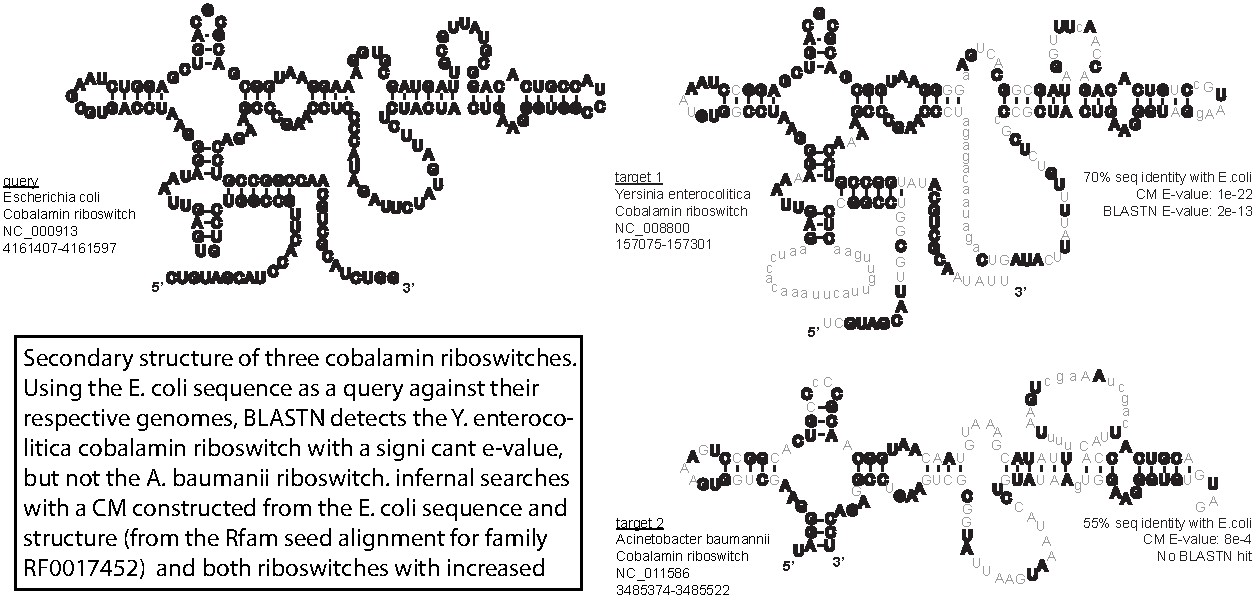
\includegraphics[width=13.5in]{figs/2013-cobalamin-poster.pdf}
\end{center}

When searching for protein coding genes, the amino acid sequence
should be used instead of the nucleotide sequence because the larger
amino acid alphabet makes protein searches much more powerful
\cite{Pearson96}.  Incorporating secondary structure into RNA searches
offers a similar boost to the statistical power of a nucleotide-only
based search for RNAs, albeit not as dramatic. Figure
\ref{fig:examples} below compares the increase in statistical
significance between BLASTN (nucleotide-based search) and BLASTP
(protein-based search) for protein-coding genes and between BLASTN
and Infernal (CM-based sequence and structure search) for RNA genes,
where both the protein-coding gene and RNA gene being searched for are
members of the same ribonucleoprotein complex.

% the caption for figure 1 (cobalamin) was in the figure.
\setcounter{figure}{1}

\begin{footnotesize}
\begin{figure}
\center{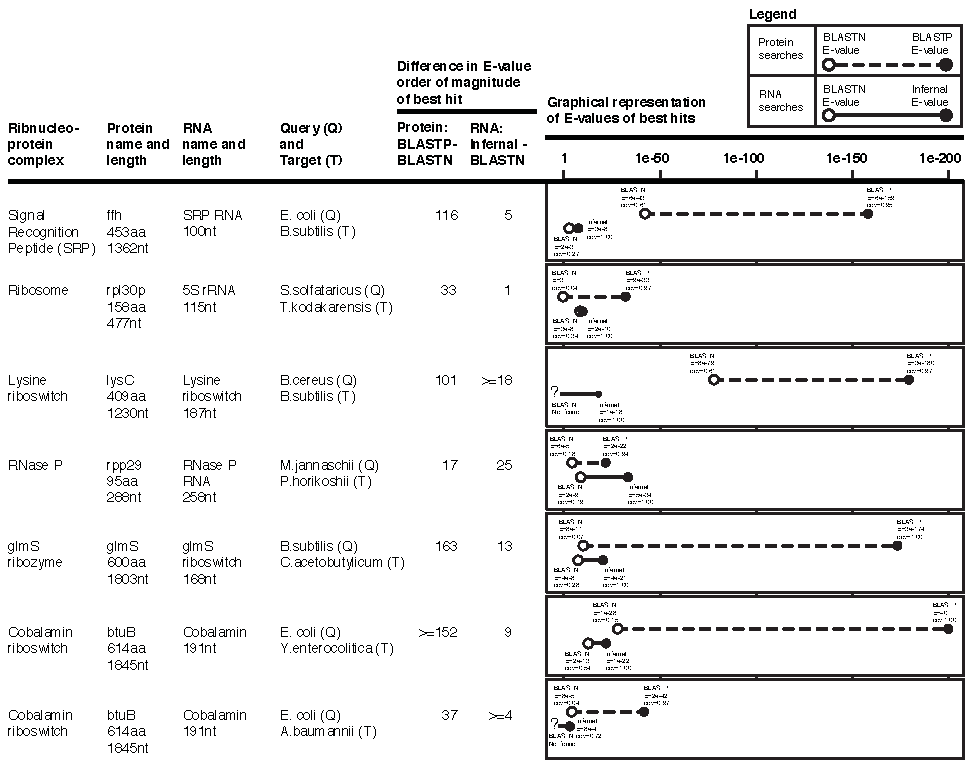
\includegraphics[width=13.5in]{figs/revised-examples}}
\caption{
Homology search improvement achieved by utilizing additional
information for proteins and structured noncoding RNAs. This figure is
from \cite{Nawrocki13b}.}
%Examples of identifying coding region homologies by amino acid sequence
%vs. nucleic acid sequence comparison (BLASTP vs. BLASTN, dashed
%lines), compared with identifying RNA homologies by primary sequence
%vs. structure/sequence comparison (BLASTN vs. infernal, solid lines)
%for several ribonucleoprotein complexes.}
%Filled circles correspond
%to BLASTP protein searches and Infernal RNA searches. Open circles
%correspond to BLASTN coding region searches and BLASTN RNA
%searches.}
%Question marks indicate targets that were not found by the
%indicated search method. Each point is labeled with its e-) and
%fractional ), calculated as the fraction of query positions included
%in the hit alignment. For each query/target
%pair, the query sequence was searched against the target genome (for
%coding sequence and rNA searches) or predicted proteome (for amino
%acid sequence searches) using the indicated search programs. For
%example, in the leftmost column, when we use the SrP protein  h in
%E. coli as a query against the B. subtilis proteome with BLASTP, the
%top scoring hit is to the  h protein with an e-value of 6 Covcoverage 10 (evalue (
\label{fig:examples}
\end{figure}
\end{footnotesize}

\columnbreak
%%%%%%%%%%%%%%%%%
% Middle column %
%%%%%%%%%%%%%%%%%

\section*{Conserved sequence and structure as statistical signals}
The conserved sequence and secondary structure of RNAs offers two
statistical signals that can be harnessed when searching
databases for homologs using CMs. In
Figure~\ref{fig:seqstructprofiles} below, the amount of information,
measured in \emph{bits}, inherent in a sequence-only profile (14
bits) and a sequence-and-structure profile (17 bits) is shown for a
toy example of an RNA family. We expect a match to a sequence-only
profile for this family once in every $2^{14}=16,384$ random
nucleotides.  Additionally modeling structure with a
sequence-and-structure based profile (like a CM) reduces this
probability 8-fold, to once every every $2^{17}=131,072$
random nucleotides.

\begin{footnotesize}
\begin{figure}
\center{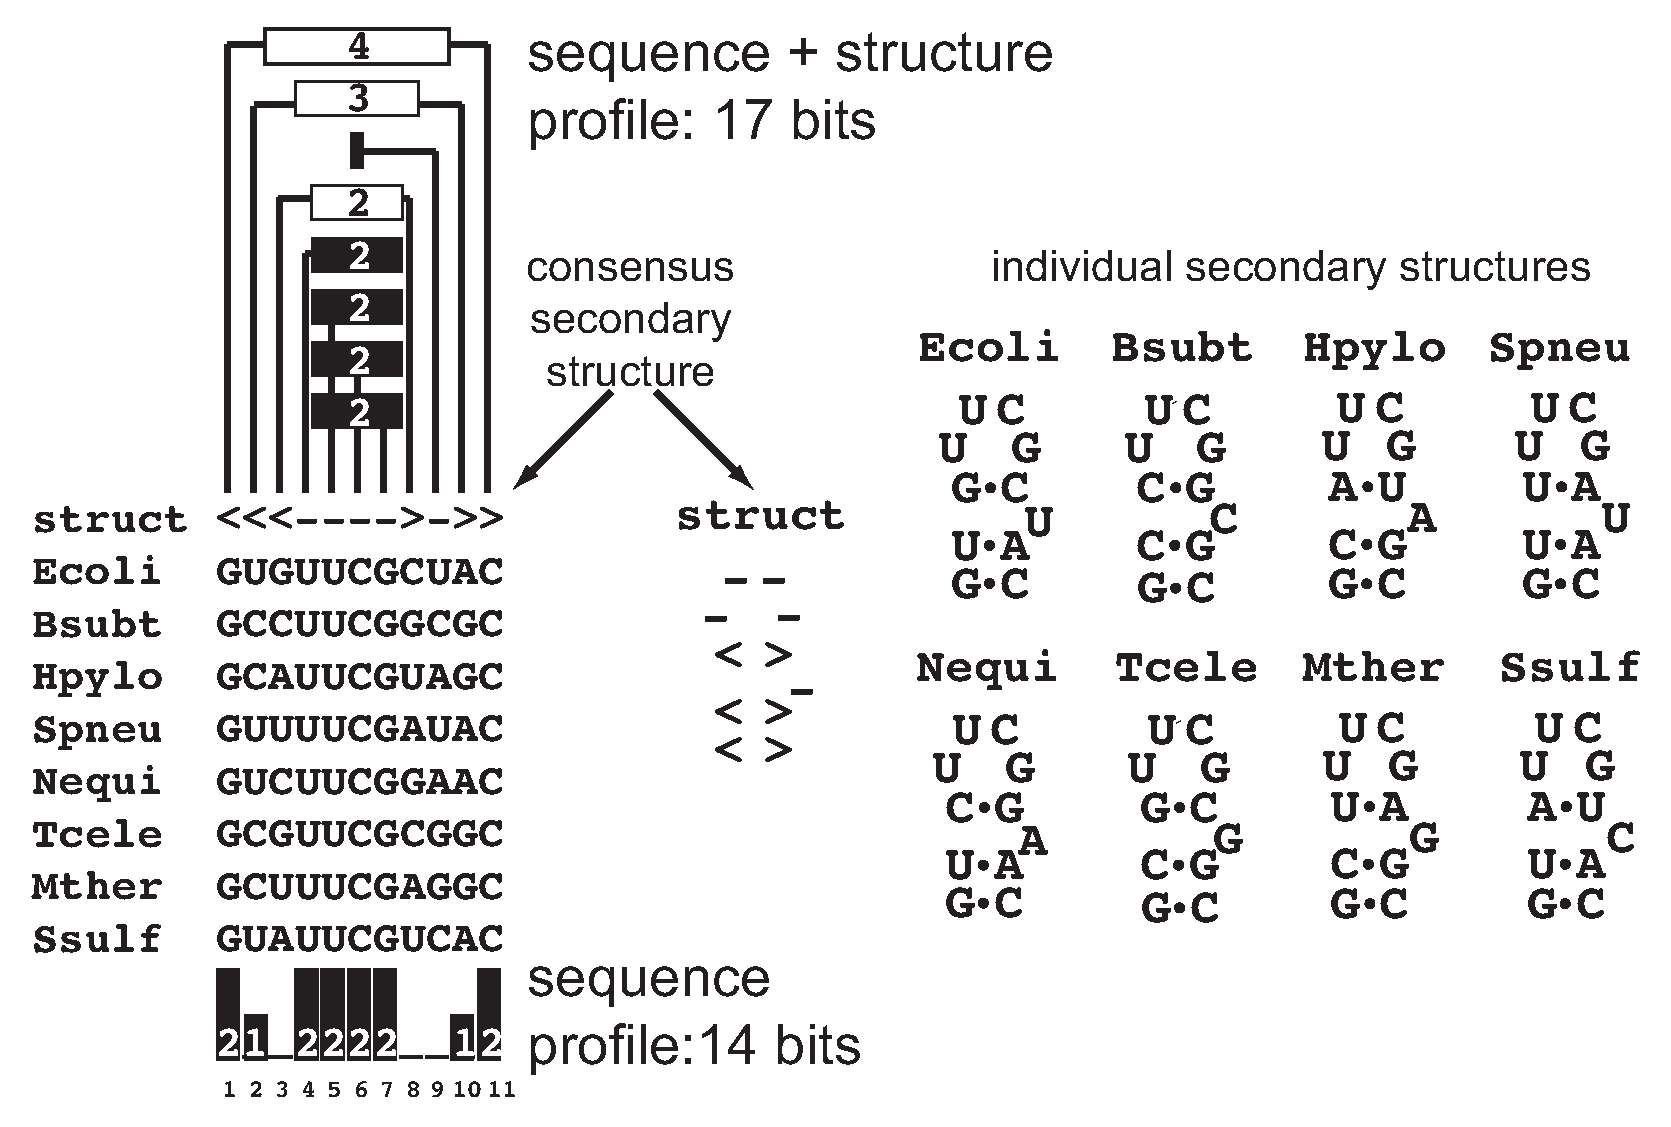
\includegraphics[width=13.5in]{figs/seqstructprofiles}}
\caption{Information in a sequence-only versus a sequence and
  structure profile. 
%The eight sequence alignment for a fabricated RNA
%  family used to build both of the profiles is on the left. 
%  The {\tt struct} line denotes the consensus secondary structure of the
%  family, with basepaired columns indicated by matching nested {\tt <}
%  and {\tt >} characters and connected by lines at top of figure. 
% The
%  structure is ignored by the sequence-only profile but used in the
%  sequence and structure profile to define dependencies between
%  basepaired columns. 
%  The eight individual secondary structures,
%  defined by imposing the consensus structure on each sequence, are
%  shown on the right. 
  Boxes with internal numbers at top and bottom of
  the alignment indicate the number of bits per position from the
  sequence (black), or per basepair from the structure (white).
  This figure is from \cite{Nawrocki13}.
}
\label{fig:seqstructprofiles}
\end{figure}
\end{footnotesize}

The amount of additional information gained from structure varies
widely for real RNA families, as shown for about 160 families in
Figure~\ref{fig:avgscores} below. 
%Some RNAs, like tRNA, include about
%as much information in their structure as in their sequence, while for
%others, the increase is relatively modest. 
Note that for most families, modeling structure
contributes at least 10 additional bits of information, which
corresponds to lowering the expected chance of a false positive in a
random database (i.e. the E-value of a database hit) by three orders
of magnitude ($2^{10} = 1024$).

\begin{footnotesize}
\begin{figure}
\center{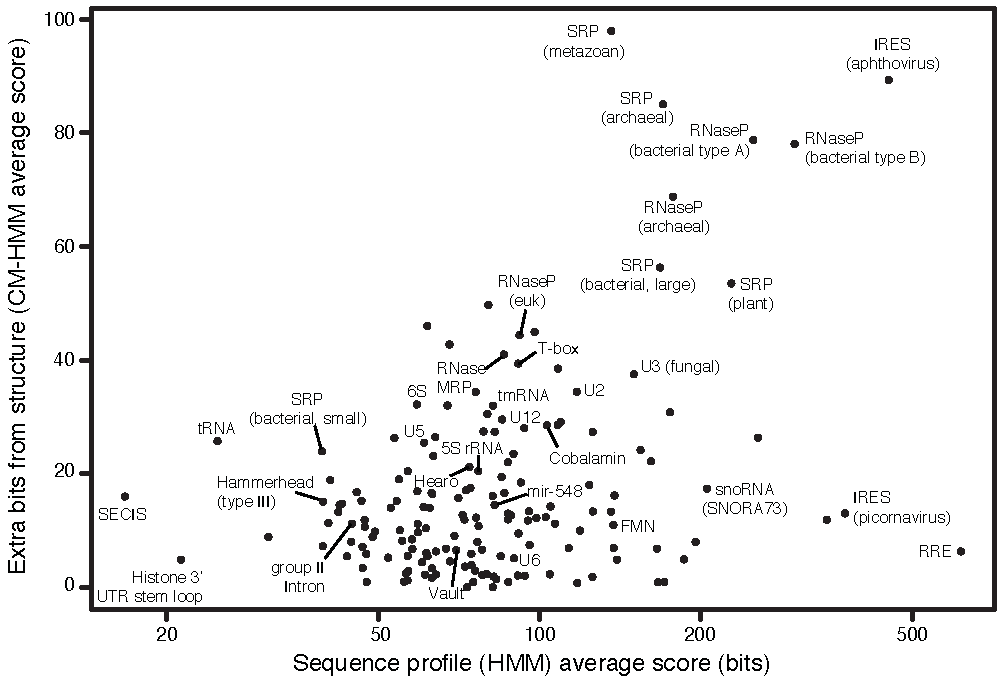
\includegraphics[width=13.5in]{figs/avgscores-rfam11}}
\caption{Additional information (in bits) gained by sequence and
  structure profiles (CMs) versus sequence-only profiles (HMMs) for
  various RNA families.  
%  Sequence and structure profiles are most
%  advantageous for families with less primary sequence information
%  (towards left) and more secondary structure information (towards
%  top), so Rfam families that gain the most from including secondary
%  structure terms in a homology search are those toward the upper left
%  quadrant. 
  Data shown for the 164 Rfam release 11.0 families
  with 50 or more sequences in the \emph{seed} alignment. For each
  family, the seed alignment was used to build two profile models, a
  CM and a profile HMM. From each model, 10,000 sequences were
  generated and scored, and the average score per sampled sequence was
  calculated. Infernal version 1.1 was used for all steps. This figure
  is from \cite{Nawrocki13b}.
%  Several of the
%  outlying points are labeled by the name of RNA family as given by
%  Rfam. Note that the x-axis is drawn on a log scale. Models were
%  built and sequences were generated and scored using Infernal version
%  1.0 programs cmbuild, cmemit and cmalign.}
}
\label{fig:avgscores}
\end{figure}
\end{footnotesize}

\columnbreak
%%%%%%%%%%%%%%%%
% Right column %
%%%%%%%%%%%%%%%%

\section*{Internal benchmark shows benefit of modeling sequence and
  structure conservation}

%As an illustrative example, I used Infernal 1.1 and Rfam CMs to annotate
%RNAs in the genome of the methanogenic archaeon
%\emph{Methanobrevibacter ruminantium} which lives in the stomachs of
%ruminant mammals such as cows. The results of searching the 102 CMs for
%Rfam families with representatives in archaea against the genome are
%given below.  Infernal finds 175 hits with E-values below $0.0098$ ($1/102$)
%from 12 different families. The GenBank annotation includes 
%66 RNAs from 4 families.

\begin{footnotesize}
\begin{figure}
\center{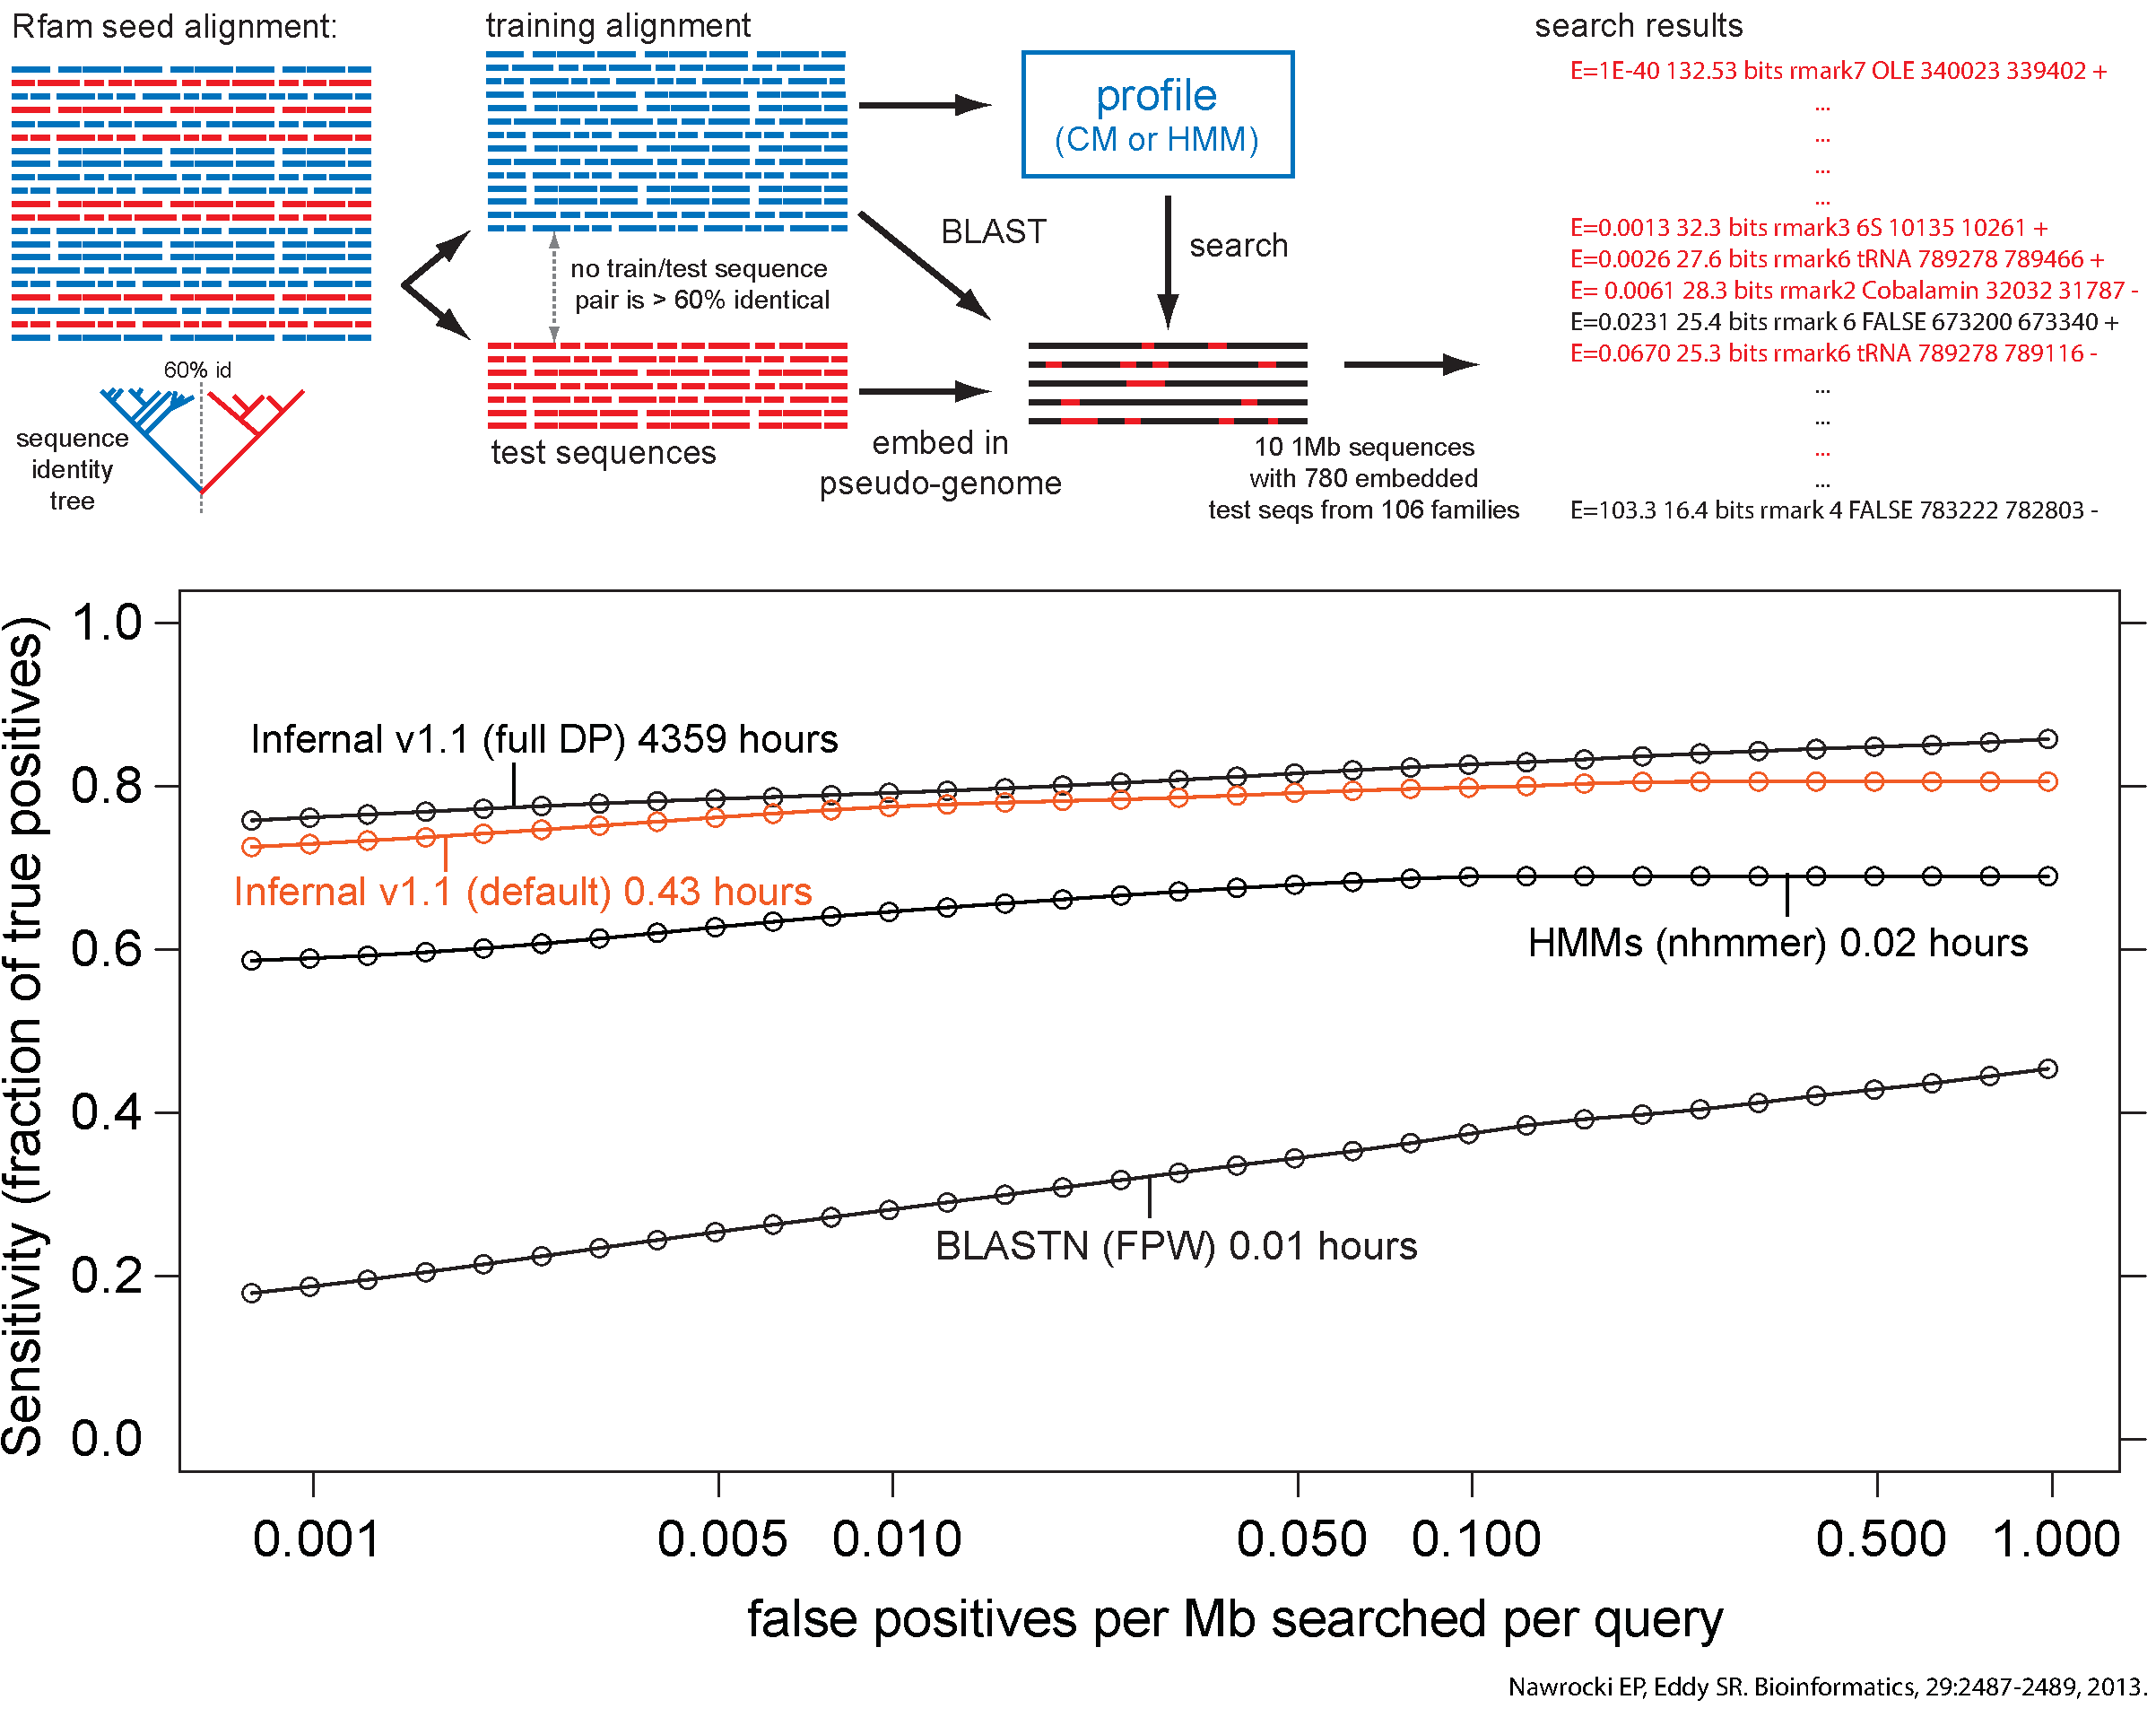
\includegraphics[width=13.5in]{figs/rmark-tree-roc-poster}}
\caption{
RMARK benchmark. Top: schematic for benchmark
construction. Bottom: Results of benchmark. Plots are shown for the new
Infernal 1.1 with and without filters, for
profile HMM searches with nhmmer \cite{Wheeler13b} (from the HMMER package included in
Infernal 1.1, default parameters) and for family-pairwise-searches
with BLASTN (ncbi-blast-2.2.28+ default parameters). The Infernal
times do not include time required for model calibration. This figure
is from \cite{Nawrocki13c}}
\label{fig:rmark}
\end{figure}
\end{footnotesize}

\vspace{0.5in}

\section*{Rfam: the RNA families database \cite{Nawrocki15}}

\begin{center}
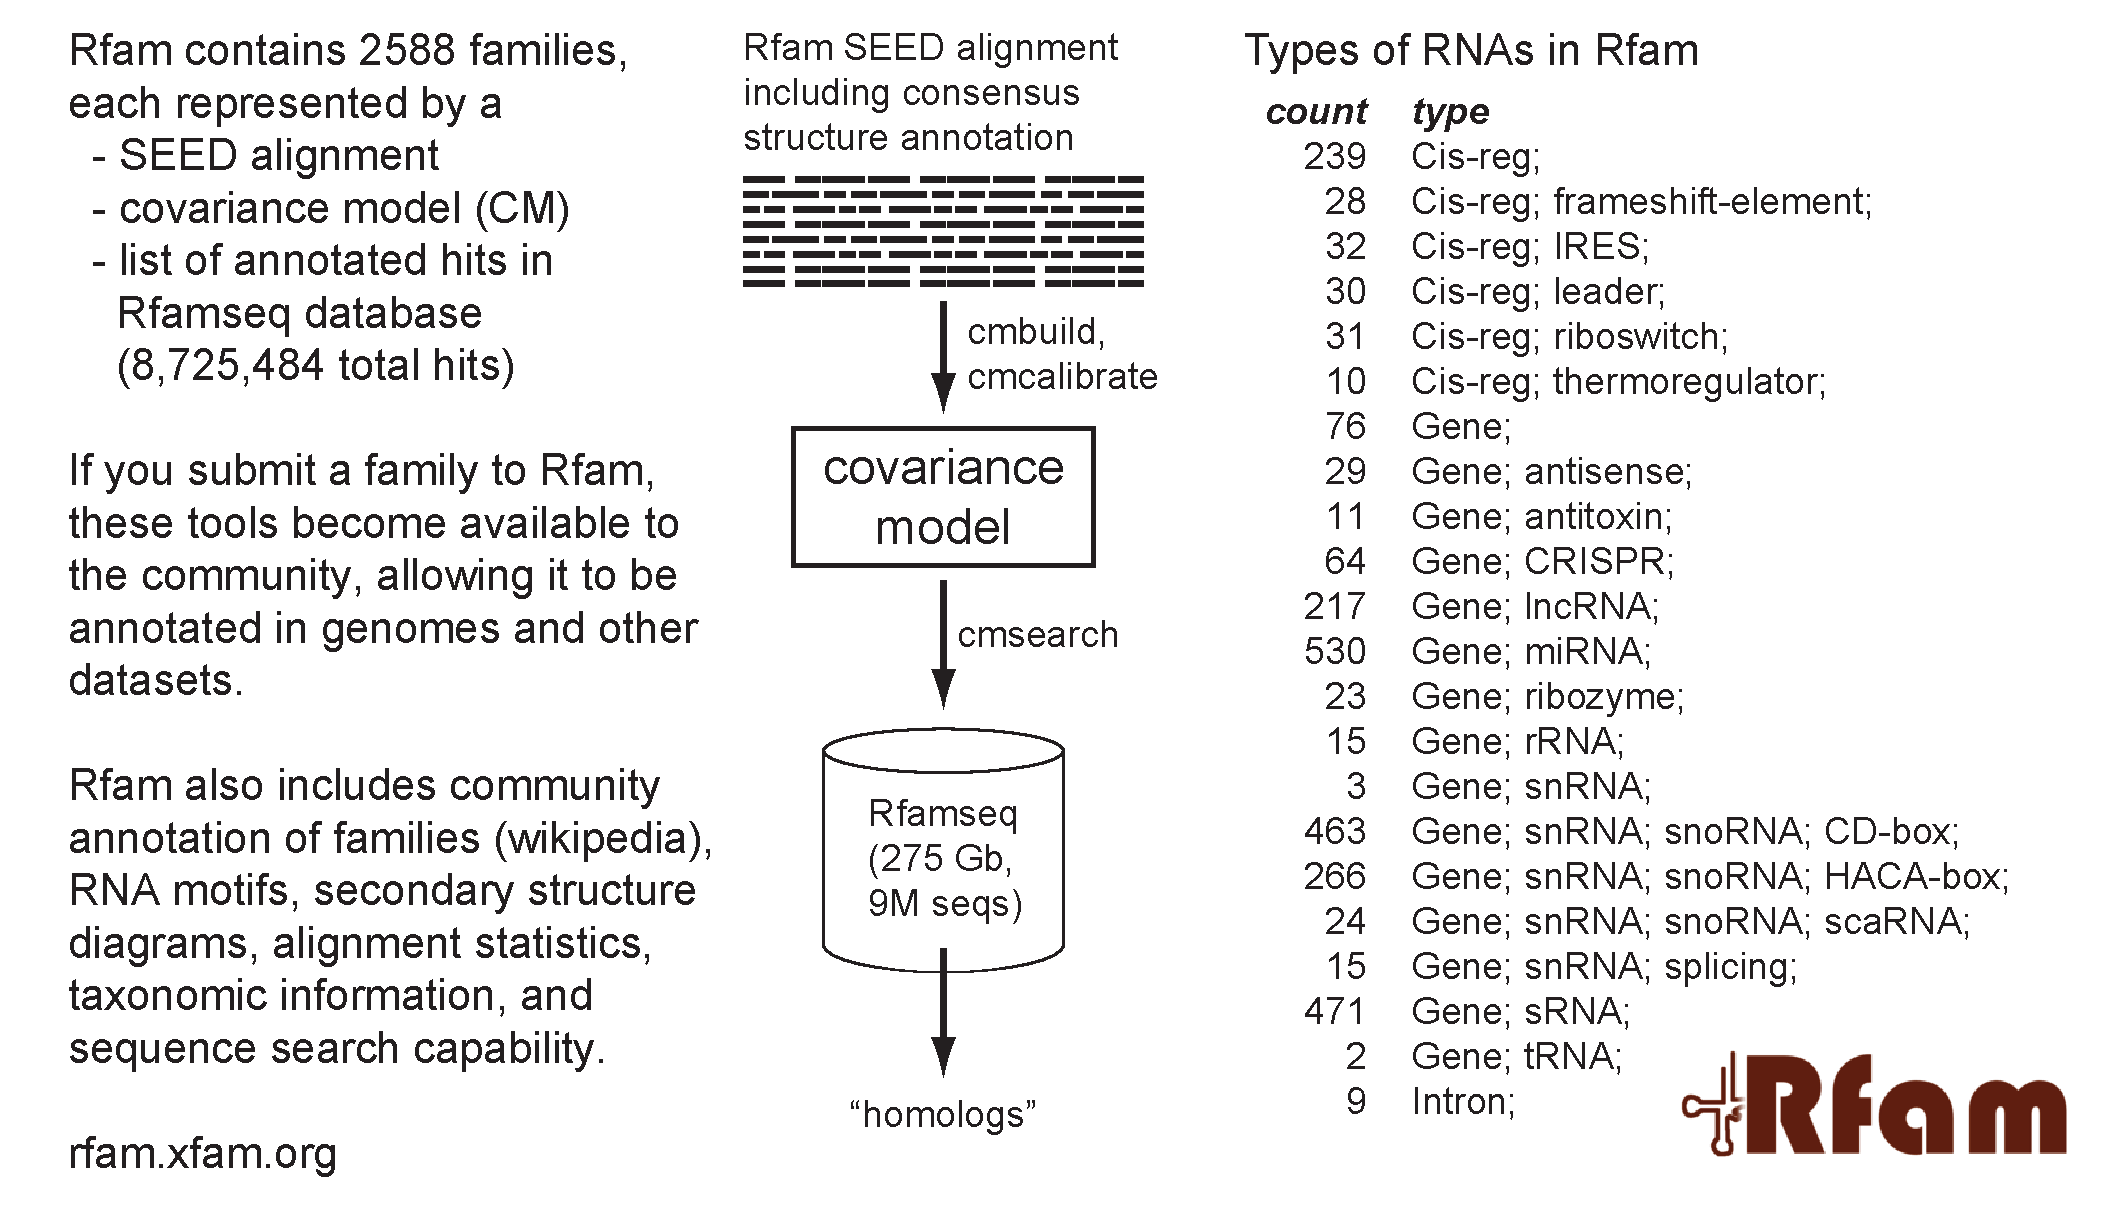
\includegraphics[width=13.5in]{figs/rfam-poster}
\end{center}

\section*{Funding}
\begin{footnotesize}
This work is supported by the Intramural Research Program of the
National Institutes of Health, National Library of Medicine (EPN), 
by Howard Hughes Medical Institute (EPN (previously), SRE), by the European
Bioinformatics institute of the European Molecular Biology Laboratory
(IK, JA, AIP), and by the Biotechnology and Biological Sciences
Research Council (IK, JA, AIP).
\end{footnotesize}

\bibliographystyle{unsrtnat}
\begin{tiny}
\bibliography{poster}
\end{tiny}

\end{multicols}

\end{document}
